\setchapterimage{fig_02}
\chapter*{TD \arabic{cptTD} :
Chasse neige \ifnormal $\star$ \else \fi \ifdifficile $\star\star$ \else \fi \iftdifficile $\star\star\star$ \else \fi
 -- \ifprof Corrigé \else Sujet \fi}
\addcontentsline{toc}{section}{TD \arabic{cptTD} : 
Chasse neige \ifnormal $\star$ \else \fi \ifdifficile $\star\star$ \else \fi \iftdifficile $\star\star\star$ \else \fi
 -- \ifprof Corrigé \else Sujet \fi}

\iflivret \stepcounter{cptTD} \else
\ifprof  \stepcounter{cptTD} \else \fi
\fi

\setcounter{question}{0}
\marginnote{D'après documents Mines-Telecom.}
\marginnote{
\UPSTIcompetence[2]{B2-14}
\UPSTIcompetence[2]{C1-05}
\UPSTIcompetence[2]{C2-07}
}

%\begin{marginfigure}
%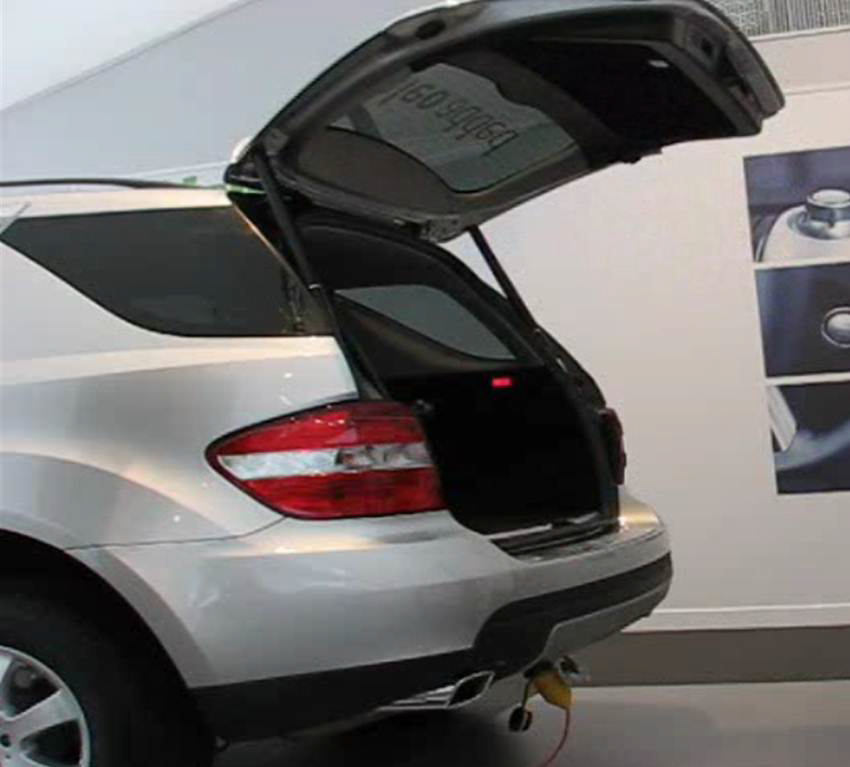
\includegraphics[width=\linewidth]{fig_00}
%\end{marginfigure}


\subsection*{Mise en situation}
\ifprof
\else
L’étrave de déneigement, objet de cette
étude, est utilisée pour dégager les routes.
Elle est composée de deux volets disposés
en « V » qui permettent d’évacuer sur les
côtés une épaisseur importante de neige.
Les deux volets sont articulés de façon
indépendante sur la pointe de l’étrave et
ont une ouverture variable contrôlée par
le conducteur à travers un vérin
d’ouverture. En fin d’utilisation ou pour
éviter des obstacles, elle est pourvue d’un
système de relevage hydraulique.

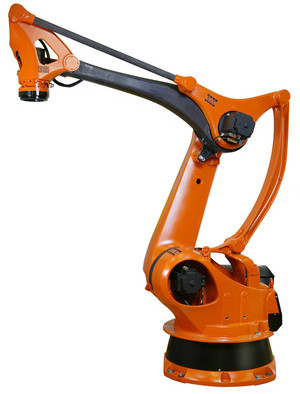
\includegraphics[width=\linewidth]{fig_01}

La pièce 7 est la lame de déneigement articulée par
rapport au châssis 3. Elle est mise en mouvement
par le vérin \{10 ; 11\}.



\subsection*{Données et hypothèses}
\begin{itemize}
\item $\gamma = \angl{x_3}{x_7}=\angl{z_3}{z_7}$ et $\beta= \angl{x_3}{x_{11}}=\angl{z_3}{z_{11}}$;
\item $\vect{z_{11}}=\vect{z_{10}}$ et $\vect{x_{11}}=\vect{x_{10}}$;
\item $\vect{HJ}=h\vect{z_7}$ et $\vect{HQ} = a\vx{3}+b\vy{3}+c\vz{3}$ et 
	$\vect{HG}=h\vect{z_7}$ et $\vect{HM}=f\vect{x_3}+g\vz{3}$.
\end{itemize}

\begin{itemize}
\item Dans le cadre de cette étude, $\beta = 37\degres$ et $\gamma = 16\degres$, $\vect{g}=-g\vect{y_3}$;
\item liaisons parfaites (pas de jeu, pas de frottement);
\item le poids de toutes les pièces est négligé, sauf celui de la pièce 7, $m_7=\SI{850}{kg}$ appliqué en $G$;
\item dimensions en mètres : $h=0,68$ ; $a=-0,33$ ; $b=0,1$; $c=1,1$ et $i=0,5$;
\item l’action de la neige sur le volet 7 est modélisée par un glisseur de moment nul en $Q$ tel que :
$\torseurstat{T}{\text{neige}}{7} =  \torseurl{Q\vx{7}}{\vect{0}}{Q}$ avec $Q = \SI{15000}{N}$;
\item le vérin d’ouverture choisi supporte une pression d'alimentation de 150 bars.
\end{itemize}



\question{Proposer une démarche permettant de vérifier si la pression d'alimentation du vérin d’ouverture est 
suffisante pour « chasser la neige ». }

